\documentclass{standalone}
\usepackage{tikz}
\usetikzlibrary{patterns, positioning}

\begin{document}
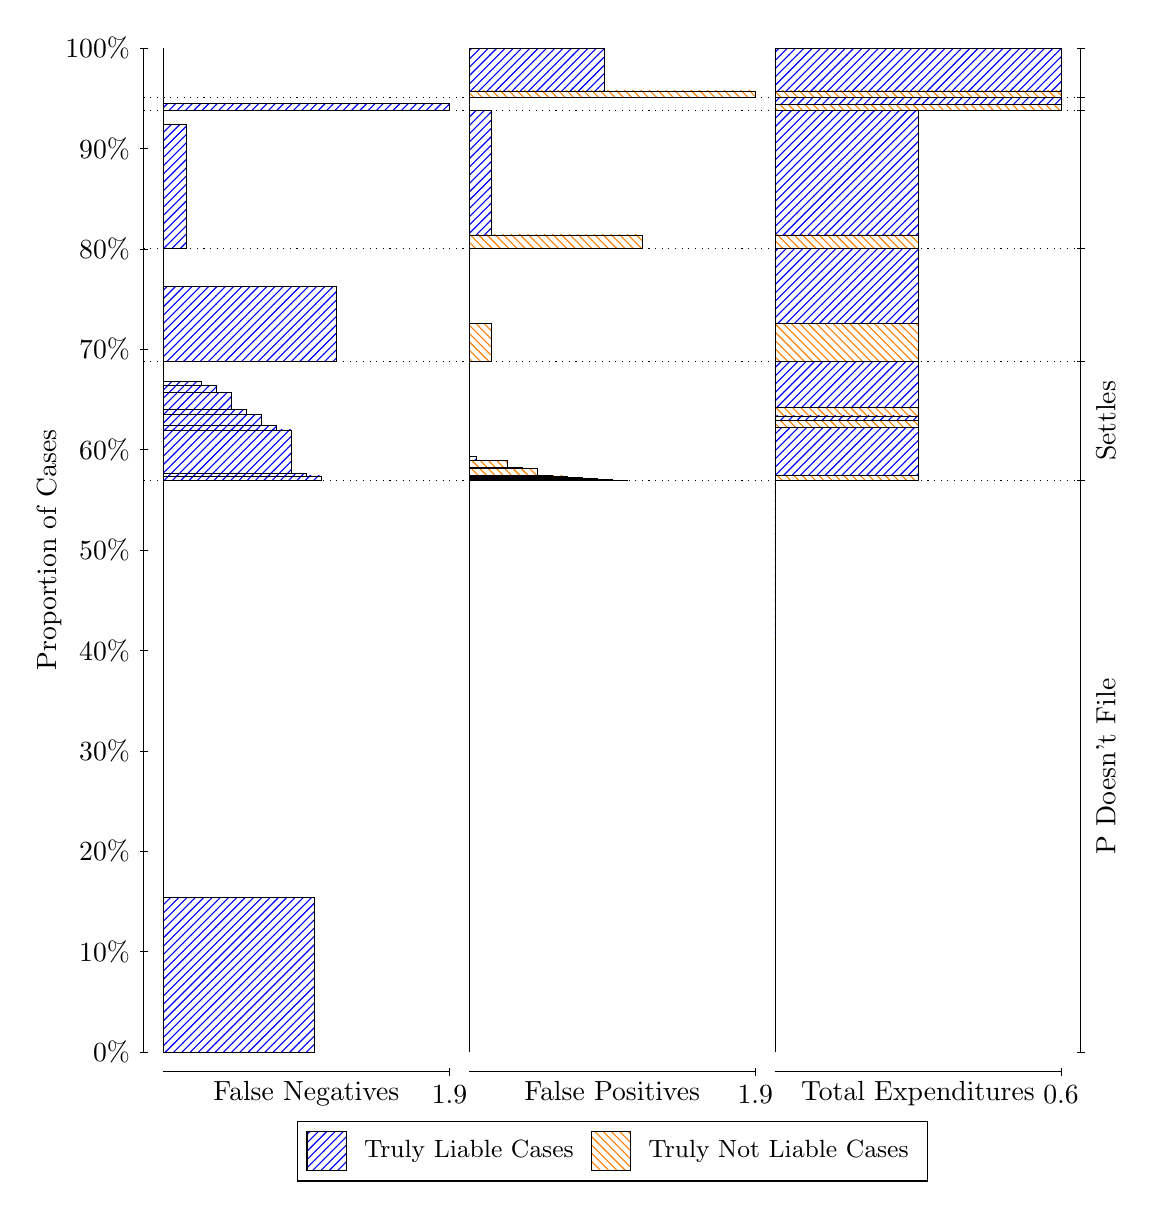
\begin{tikzpicture}
\draw[black, very thin] (1.5,1.75) -- (1.5,14.5);
\node[rotate=90, anchor=center] at (0.3, 8.125) {Proportion of Cases};
\draw[black, very thin] (1.45,1.75) -- (1.55,1.75);
\node[anchor=east] at (1.45, 1.75) {0\%};
\draw[black, very thin] (1.45,3.025) -- (1.55,3.025);
\node[anchor=east] at (1.45, 3.025) {10\%};
\draw[black, very thin] (1.45,4.3) -- (1.55,4.3);
\node[anchor=east] at (1.45, 4.3) {20\%};
\draw[black, very thin] (1.45,5.575) -- (1.55,5.575);
\node[anchor=east] at (1.45, 5.575) {30\%};
\draw[black, very thin] (1.45,6.85) -- (1.55,6.85);
\node[anchor=east] at (1.45, 6.85) {40\%};
\draw[black, very thin] (1.45,8.125) -- (1.55,8.125);
\node[anchor=east] at (1.45, 8.125) {50\%};
\draw[black, very thin] (1.45,9.4) -- (1.55,9.4);
\node[anchor=east] at (1.45, 9.4) {60\%};
\draw[black, very thin] (1.45,10.675) -- (1.55,10.675);
\node[anchor=east] at (1.45, 10.675) {70\%};
\draw[black, very thin] (1.45,11.95) -- (1.55,11.95);
\node[anchor=east] at (1.45, 11.95) {80\%};
\draw[black, very thin] (1.45,13.225) -- (1.55,13.225);
\node[anchor=east] at (1.45, 13.225) {90\%};
\draw[black, very thin] (1.45,14.5) -- (1.55,14.5);
\node[anchor=east] at (1.45, 14.5) {100\%};

\draw[black, very thin] (13.4,1.75) -- (13.4,14.5);
\draw[black, very thin] (13.35,1.75) -- (13.45,1.75);
\node[anchor=west] at (13.35, 1.75) {};
\draw[black, very thin] (13.35,9.0056) -- (13.45,9.0056);
\node[anchor=west] at (13.35, 9.0056) {};
\draw[black, very thin] (13.35,10.523) -- (13.45,10.523);
\node[anchor=west] at (13.35, 10.523) {};
\draw[black, very thin] (13.35,11.952) -- (13.45,11.952);
\node[anchor=west] at (13.35, 11.952) {};
\draw[black, very thin] (13.35,13.707) -- (13.45,13.707);
\node[anchor=west] at (13.35, 13.707) {};
\draw[black, very thin] (13.35,13.87) -- (13.45,13.87);
\node[anchor=west] at (13.35, 13.87) {};
\draw[black, very thin] (13.35,14.5) -- (13.45,14.5);
\node[anchor=west] at (13.35, 14.5) {};

\draw[black, very thin, pattern color=blue, pattern=north east lines] (1.75,1.75) rectangle (3.6623,3.7121);
\draw[black, very thin, pattern color=orange, pattern=north west lines] (1.75,3.7121) rectangle (1.75,9.0056);
\draw[black, very thin, pattern color=blue, pattern=north east lines] (1.75,9.0056) rectangle (3.7579,9.0666);
\draw[black, very thin, pattern color=blue, pattern=north east lines] (1.75,9.0666) rectangle (3.5667,9.0976);
\draw[black, very thin, pattern color=blue, pattern=north east lines] (1.75,9.0976) rectangle (3.3754,9.6495);
\draw[black, very thin, pattern color=blue, pattern=north east lines] (1.75,9.6495) rectangle (3.1842,9.7069);
\draw[black, very thin, pattern color=blue, pattern=north east lines] (1.75,9.7069) rectangle (2.993,9.8516);
\draw[black, very thin, pattern color=blue, pattern=north east lines] (1.75,9.8516) rectangle (2.8018,9.909);
\draw[black, very thin, pattern color=blue, pattern=north east lines] (1.75,9.909) rectangle (2.6105,10.131);
\draw[black, very thin, pattern color=blue, pattern=north east lines] (1.75,10.131) rectangle (2.4193,10.218);
\draw[black, very thin, pattern color=blue, pattern=north east lines] (1.75,10.218) rectangle (2.2281,10.264);
\draw[black, very thin, pattern color=orange, pattern=north west lines] (1.75,10.264) rectangle (1.75,10.523);
\draw[black, very thin, pattern color=blue, pattern=north east lines] (1.75,10.523) rectangle (3.9491,11.47);
\draw[black, very thin, pattern color=orange, pattern=north west lines] (1.75,11.47) rectangle (1.75,11.952);
\draw[black, very thin, pattern color=blue, pattern=north east lines] (1.75,11.952) rectangle (2.0368,13.533);
\draw[black, very thin, pattern color=orange, pattern=north west lines] (1.75,13.533) rectangle (1.75,13.707);
\draw[black, very thin, pattern color=blue, pattern=north east lines] (1.75,13.707) rectangle (5.3833,13.792);
\draw[black, very thin, pattern color=orange, pattern=north west lines] (1.75,13.792) rectangle (1.75,13.87);
\draw[black, very thin, pattern color=orange, pattern=north west lines] (1.75,13.87) rectangle (1.75,13.957);
\draw[black, very thin, pattern color=blue, pattern=north east lines] (1.75,13.957) rectangle (1.75,14.5);
\draw[black, very thin, pattern color=orange, pattern=north west lines] (5.6333,1.75) rectangle (5.6333,7.0435);
\draw[black, very thin, pattern color=blue, pattern=north east lines] (5.6333,7.0435) rectangle (5.6333,9.0056);
\draw[black, very thin, pattern color=orange, pattern=north west lines] (5.6333,9.0056) rectangle (7.6412,9.009);
\draw[black, very thin, pattern color=orange, pattern=north west lines] (5.6333,9.009) rectangle (7.45,9.017);
\draw[black, very thin, pattern color=orange, pattern=north west lines] (5.6333,9.017) rectangle (7.2588,9.0383);
\draw[black, very thin, pattern color=orange, pattern=north west lines] (5.6333,9.0383) rectangle (7.0675,9.0458);
\draw[black, very thin, pattern color=orange, pattern=north west lines] (5.6333,9.0458) rectangle (6.8763,9.0656);
\draw[black, very thin, pattern color=orange, pattern=north west lines] (5.6333,9.0656) rectangle (6.6851,9.0715);
\draw[black, very thin, pattern color=orange, pattern=north west lines] (5.6333,9.0715) rectangle (6.6851,9.0735);
\draw[black, very thin, pattern color=orange, pattern=north west lines] (5.6333,9.0735) rectangle (6.4939,9.164);
\draw[black, very thin, pattern color=orange, pattern=north west lines] (5.6333,9.164) rectangle (6.3026,9.1751);
\draw[black, very thin, pattern color=orange, pattern=north west lines] (5.6333,9.1751) rectangle (6.1114,9.2651);
\draw[black, very thin, pattern color=blue, pattern=north east lines] (5.6333,9.2651) rectangle (5.7289,9.3102);
\draw[black, very thin, pattern color=blue, pattern=north east lines] (5.6333,9.3102) rectangle (5.6333,10.523);
\draw[black, very thin, pattern color=orange, pattern=north west lines] (5.6333,10.523) rectangle (5.9202,11.005);
\draw[black, very thin, pattern color=blue, pattern=north east lines] (5.6333,11.005) rectangle (5.6333,11.952);
\draw[black, very thin, pattern color=orange, pattern=north west lines] (5.6333,11.952) rectangle (7.8325,12.127);
\draw[black, very thin, pattern color=blue, pattern=north east lines] (5.6333,12.127) rectangle (5.9202,13.707);
\draw[black, very thin, pattern color=orange, pattern=north west lines] (5.6333,13.707) rectangle (5.6333,13.786);
\draw[black, very thin, pattern color=blue, pattern=north east lines] (5.6333,13.786) rectangle (5.6333,13.87);
\draw[black, very thin, pattern color=orange, pattern=north west lines] (5.6333,13.87) rectangle (9.2667,13.957);
\draw[black, very thin, pattern color=blue, pattern=north east lines] (5.6333,13.957) rectangle (7.3544,14.5);
\draw[black, very thin, pattern color=orange, pattern=north west lines] (9.5167,1.75) rectangle (9.5167,7.0435);
\draw[black, very thin, pattern color=blue, pattern=north east lines] (9.5167,7.0435) rectangle (9.5167,9.0056);
\draw[black, very thin, pattern color=orange, pattern=north west lines] (9.5167,9.0056) rectangle (11.333,9.0715);
\draw[black, very thin, pattern color=blue, pattern=north east lines] (9.5167,9.0715) rectangle (11.333,9.6784);
\draw[black, very thin, pattern color=orange, pattern=north west lines] (9.5167,9.6784) rectangle (11.333,9.7684);
\draw[black, very thin, pattern color=blue, pattern=north east lines] (9.5167,9.7684) rectangle (11.333,9.8294);
\draw[black, very thin, pattern color=orange, pattern=north west lines] (9.5167,9.8294) rectangle (11.333,9.933);
\draw[black, very thin, pattern color=blue, pattern=north east lines] (9.5167,9.933) rectangle (11.333,10.523);
\draw[black, very thin, pattern color=orange, pattern=north west lines] (9.5167,10.523) rectangle (11.333,11.005);
\draw[black, very thin, pattern color=blue, pattern=north east lines] (9.5167,11.005) rectangle (11.333,11.952);
\draw[black, very thin, pattern color=orange, pattern=north west lines] (9.5167,11.952) rectangle (11.333,12.127);
\draw[black, very thin, pattern color=blue, pattern=north east lines] (9.5167,12.127) rectangle (11.333,13.707);
\draw[black, very thin, pattern color=orange, pattern=north west lines] (9.5167,13.707) rectangle (13.15,13.786);
\draw[black, very thin, pattern color=blue, pattern=north east lines] (9.5167,13.786) rectangle (13.15,13.87);
\draw[black, very thin, pattern color=orange, pattern=north west lines] (9.5167,13.87) rectangle (13.15,13.957);
\draw[black, very thin, pattern color=blue, pattern=north east lines] (9.5167,13.957) rectangle (13.15,14.5);
\draw[black, dotted] (1.5,9.0056) -- (13.4,9.0056);
\draw[black, dotted] (1.5,10.523) -- (13.4,10.523);
\draw[black, dotted] (1.5,11.952) -- (13.4,11.952);
\draw[black, dotted] (1.5,13.707) -- (13.4,13.707);
\draw[black, dotted] (1.5,13.87) -- (13.4,13.87);
\draw[black, very thin] (1.75,1.5) -- (5.3833,1.5);
\node[anchor=north] at (3.5667, 1.5) {False Negatives};
\draw[black, very thin] (5.3833,1.45) -- (5.3833,1.55);
\node[anchor=north] at (5.3833, 1.45) {1.9};

\draw[black, very thin] (5.6333,1.5) -- (9.2667,1.5);
\node[anchor=north] at (7.45, 1.5) {False Positives};
\draw[black, very thin] (9.2667,1.45) -- (9.2667,1.55);
\node[anchor=north] at (9.2667, 1.45) {1.9};

\draw[black, very thin] (9.5167,1.5) -- (13.15,1.5);
\node[anchor=north] at (11.333, 1.5) {Total Expenditures};
\draw[black, very thin] (13.15,1.45) -- (13.15,1.55);
\node[anchor=north] at (13.15, 1.45) {0.6};

\node[black, centered, rotate=90] at (13.72, 5.3778) {P Doesn't File};
\node[black, centered, rotate=90] at (13.72, 9.7643) {Settles};





\draw (7.449999999999999,1.5) node[draw=none] (baseCoordinate) {};
\begin{scope}[align=center]
        \matrix[scale=0.5, draw=black, below=0.5cm of baseCoordinate, nodes={draw}, column sep=0.1cm]{
            \node[rectangle, draw, minimum width=0.5cm, minimum height=0.5cm, pattern=north east lines, pattern color=blue] {}; &
            \node[draw=none, font=\small] (B) {Truly Liable Cases}; &
            \node[rectangle, draw, minimum width=0.5cm, minimum height=0.5cm, pattern=north west lines, pattern color=orange] {}; &
            \node[draw=none, font=\small] (B) {Truly Not Liable Cases}; \\
            };
\end{scope}

\end{tikzpicture}
\end{document}